\chapter{Implementation}

\section{Applying Aspect}

The first implementation detail I have to tackle is how the various aspects are applied to a given method. What I really needed is a way to mark a given method, signaling to Buffalo that this method is special, that its IL instructions need to be modified. Since Buffalo is only working with assembly, there need to be a way to encode that information in the metadata of the assembly. System.Attribute does fits the bill perfectly in this regard.

System.Attribute is used to provide additional information about class members. When we compile the source code, it is converted into Microsoft Intermediate Language (MSIL) and put inside a portable executable (PE) file, with the metadata generated by the compiler. We can take advantage of this behavior to encode our aspect in MSIL and later be processed by Buffalo.

This means that all the Buffalo aspects subclass System.Attribute, therefore all Buffalo aspects are in fact just a special type of attribute that is understood by Buffalo. Like any regular attributes, the aspects can be applied in three level:

1. Method level - an individual method.
2. Class level - if applied to a class, all public methods including the public properties automatically get applied.
3. Assembly level - if applied to an assembly, \#2 will apply but for all the [public?] classes within the assembly.

The Buffalo aspects can also be excluded on any given level, if so the target method will be skipped over. No matter how the aspect attributes are applied, ultimately they will result in a list of the methods that will be annotated. This simply mean if the aspect is applied to a single method, that method is the only one that will get MSIL modified. If the aspect is applied on the whole assembly, then all public methods will be MSIL modified.

To get the list of the eligible methods for MSIL modification, Buffalo attempts various checking according to figure~\ref{logical_inclusion} to see if it should include a given method.

\begin{figure}[here]
  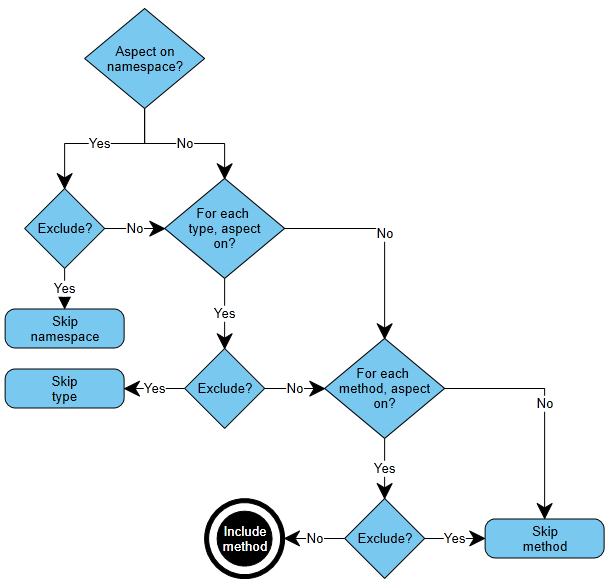
\includegraphics[scale=1.0]{AspectLogicalInclusion.PNG}
  \centering
  \caption{Logical inclusion\label{logical_inclusion}}
\end{figure}

The above logic diagram checks if an aspect is applied, if yes then check if the it is set to be excluded. If the aspect is applied on the assembly level, then Buffalo simply apply the aspect to every public methods in every class within the same assembly.

If no aspect is applied on the assembly, that does not necessarily mean no aspect is applied anywhere, the aspect might still be applied on the class or method level. Buffalo will go through each class type, if aspect is found, then it will apply the aspect to all the class’s public methods.

If aspect is not on assembly or the class level, Buffalo checks each method to determine if it should be applied.

\section{Aspect Interface}

Figure~\ref{uml01} depicts part of the system, where it shows how we can use it to find aspects during reflection.

\begin{figure}[here]
  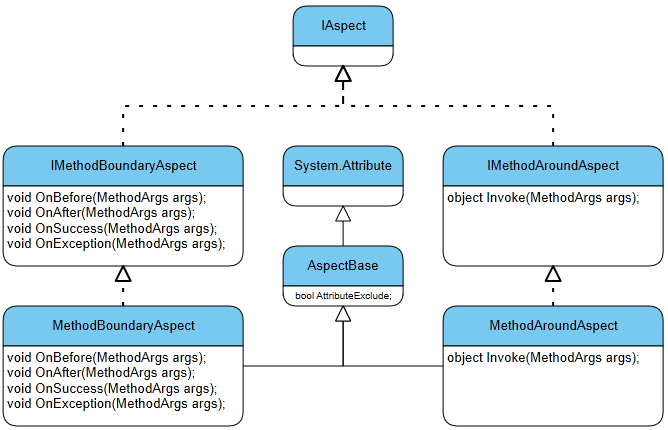
\includegraphics[scale=1.0]{Uml01.PNG}
  \centering
  \caption{Logical inclusion\label{uml01}}
\end{figure}

All aspects ultimately implements the IAspect interface, therefore we can conclude that for all the types in an assembly, if it implements IAspect, then it must be an aspect itself.

All aspects have a property named AttributeExclude, if set to true then the annotated assembly, class or method will not be included in the weaving.

Another design decision is that more than one aspect can be applied at any given level. This will allow developers more flexibility while developing multiple aspects and apply them as needed.

Furthermore, by default, all the aspects themselves will be ignored. This is to prevent an aspect from applying to itself, which will cause stack overflow in some cases. Although an aspect should be able to be applied to a different aspect in theory, however this is not implemented in Buffalo, nevertheless this is something to think about in the future work.

Another point worth mentioning is that when developing an aspect, the developer can access some information about the annotated method, such as the method signature, return type, list of parameters passed into the method and their respective values. We will look at some example later on.

\section{Implementation Overview}

The overall implementation process can be illustrated as figure~\ref{implementation_overview}, where the first step of finding all eligible methods using the logical diagram mentioned in figure~\ref{logical_inclusion}.

\begin{figure}[here]
  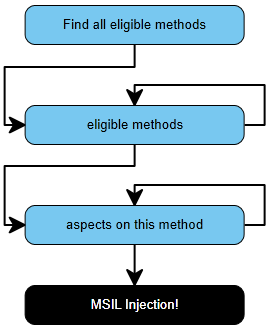
\includegraphics[scale=1.0]{ImplementationOverview3.PNG}
  \centering
  \caption{Logical inclusion\label{implementation_overview}}
\end{figure}

The actual injection phrase will be depending on the type of aspect, as we mentioned above currently Buffalo supports the Boundary aspects where various point of execution can be intercepted, and the Around aspect where a method can be completely replaced.

\section{MethodBoundaryAspect Implementation Detail}

Each type of aspect has its own injector that implements the IInjectable interface. This interface contains only one method contract - Inject(..). It takes the list of eligible methods and inject the appropriate aspect to them.

The Boundary aspect is pretty straightforward to implement, take the following hello world example, wrapped in a try..catch..finally block as we mentioned above:

\begin{lstlisting}[caption={SayHello function}, label=sayhello]
public void SayHello()
{
   try{
       Console.WriteLine(“Hello World!”);
   }catch(Exception ex){
   }finally{
   }
}
\end{lstlisting}

If we look at the generated MSIL shown in figure~\ref{methodboundary01}(Note that I have cleaned up the MSIL a bit for easy display):

\begin{figure}[here]
  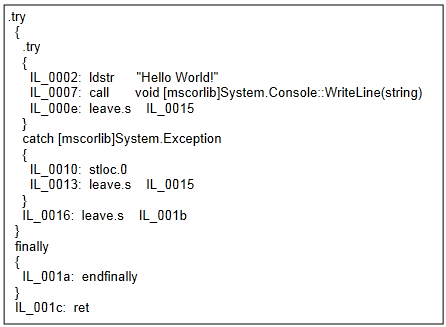
\includegraphics[scale=1.0]{MethodBoundaryOverviewB4.PNG}
  \centering
  \caption{MSIL before\label{methodboundary01}}
\end{figure}

This is the standard emission of the CLR. In CLR there is a concept of the protected region, where each region is associated with a handler. A try-catch-finally is actually encapsulated in two such regions: a catch and a finally. From here we can easily figure out where to inject our aspect, as shown in the following figure~\ref{methodboundary02}

\begin{figure}[here]
  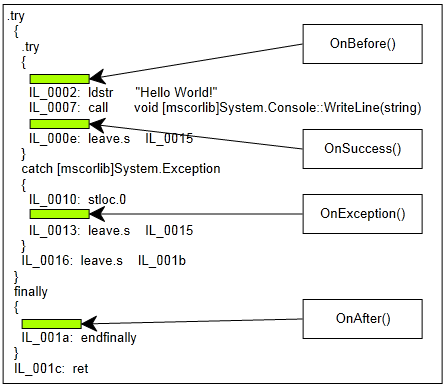
\includegraphics[scale=1.0]{MethodBoundaryOverview.PNG}
  \centering
  \caption{MSIL interception points\label{methodboundary02}}
\end{figure}

\section{MethodAroundAspect Implementation Detail}

The Around aspect on the other hand is a much more complicated compared to the Boundary aspect.

MethodAroundAspect implements IMethodAroundAspect that has the following contract:

void Invoke(MethodArgs arg)

From a developer’s perspective, when writing an aspect, he can issue a Proceed() to signal a call back into the original method. The steps taken to implement Around in MSIL is roughly as follow:

1. Create a replacement for the annotated function.
2. Create and store a variable pointing to the aspect.
3. Copy all parameters from original method to the newly created replacement function.
4. Create a variable to hold MethodArgs.
5. Issue a call to Invoke() from the replacement function, passing in the MethodArgs variable.
6. Handle the return value appropriately.
   6a. If original method returns non void type, store the return value appropriately.
   6b. If original method returns void, we need to discard the return value from Invoke()
7. Handle Proceed() that might be issued from inside the Invoke()
   7a. Load all the parameters onto the stack.
   7b. Call back into the original method.
   7c. Handle the return value appropriately.
8. Modify all calls from original method to the replacement method.

As figure~\ref{around_overview} shown, the actual calling of either the original or replacement method is abstracted away. This is also a testament of the saying in Software Engineering that “Anything can be resolved by another layer of abstraction”.

\section{MethodArgs}

Another early decision was that from a given aspect, developer must be able to access information about the annotated method. Details such as the name of the method; its signature and return type. Also the list of parameters that are being passed into the method including type, name and value.

Being able to capture some information about the annotated methods will be useful. For example, if we create a trace aspect to perform profiling, we can output all those information about the method at the time it was access. Being able to look at the parameter values in case of error will also be extremely useful in case of debugging.

To achieve the above MethodArgs is used. This is the object passed into each aspect. During the weaving, an instance of MethodArgs is injected into each method, with all properties assembled dynamically to capture the information of the current method.

At first each OnBefore, OnSuccess, OnException and OnAfter has its own distinct MethodArgs object passed into them. Later on as an optimization only one instance is instantiated at the beginning of the method body and that instance is used in all the MethodBoundaryAspect.

[Example?]

\section{Solution Structure}

Originally Buffalo was in one executable, that includes the various aspects and the program that initiate the weaving. It was later on splitted into two assembly, one is the actual implementation as a DLL, another is just a command line executable that calls into the DLL to perform the weaving. This separation is necessary so developer can perform weaving from the command line or hook into MSBuild if necessary. To actually write the aspect, developer only need to reference the DLL which is much cleaner than referencing an executable.
%
%\begin{itemize}
%\item{} Software details (use as many section as needed for class design, 
%database tables, middleware, etc.)

%\item{} Make sure you present and comment on any interesting issues about
%your implementation that you are proud of or unhappy with

%\item{} Skip code listing and specific UML diagrams, etc. to an appendix

%\end{itemize}
%
